\documentclass{scrartcl}
\usepackage[mathletters]{ucs}
\usepackage[utf8x]{inputenc}
\usepackage{amssymb}
\usepackage{amsmath}
\usepackage[usenames]{color}
\usepackage{hyperref}
\usepackage{wasysym}
\usepackage{graphicx}
\usepackage[normalem]{ulem}
\usepackage{enumerate}

\usepackage{listings}

\lstset{ %
basicstyle=\footnotesize,       % the size of the fonts that are used for the code
showspaces=false,               % show spaces adding particular underscores
showstringspaces=false,         % underline spaces within strings
showtabs=false,                 % show tabs within strings adding particular underscores
frame=single,                   % adds a frame around the code
tabsize=2,                      % sets default tabsize to 2 spaces
breaklines=true,                % sets automatic line breaking
breakatwhitespace=false,        % sets if automatic breaks should only happen at whitespace
}


\title{Masterproef Tool Wear Inspection - Update 2 DH}
\date{dinsdag 08 december 2020}
\author{}

\begin{document}

\maketitle

		\section{Masterproef Tool Wear Inspection - Update 2 DH}

Created vrijdag 20 november 2020



\subsection{Mail}

Beste meneer Hulens,

 

Een nieuwe update over mijn masterproef over Tool Wear Inspection.

Hieronder een overzicht van wat ik heb gedaan, wat ik zal doen en een korte samenvatting van wat we vorige keer hebben besproken.

 

Wat ik afgelopen week heb gedaan:

Opstelling maken

Een simpele setup bepalen om snel te zien wat de plaatjes doen met het invallende licht en hoe dit op de camera overkomt. Hierbij kwam ik al op vrij goede resultaten voor de belichting door een bureaulamp horizontaal te laten schijnen op het plaatje. Hier is een foto van te vinden in de bijlage. Hier staat ook het licht van de camera nog aan, wanneer dit wordt uitgeschakeld is de fout mooi in het oranje te zien en is de achtergrond vrij donker (te zien in bijlage).





\href{./Masterproef_Tool_Wear_Inspection_-_Update_2_DH/pasted_image.tiff}{./Masterproef_Tool_Wear_Inspection_-_Update_2_DH/pasted_image.tiff}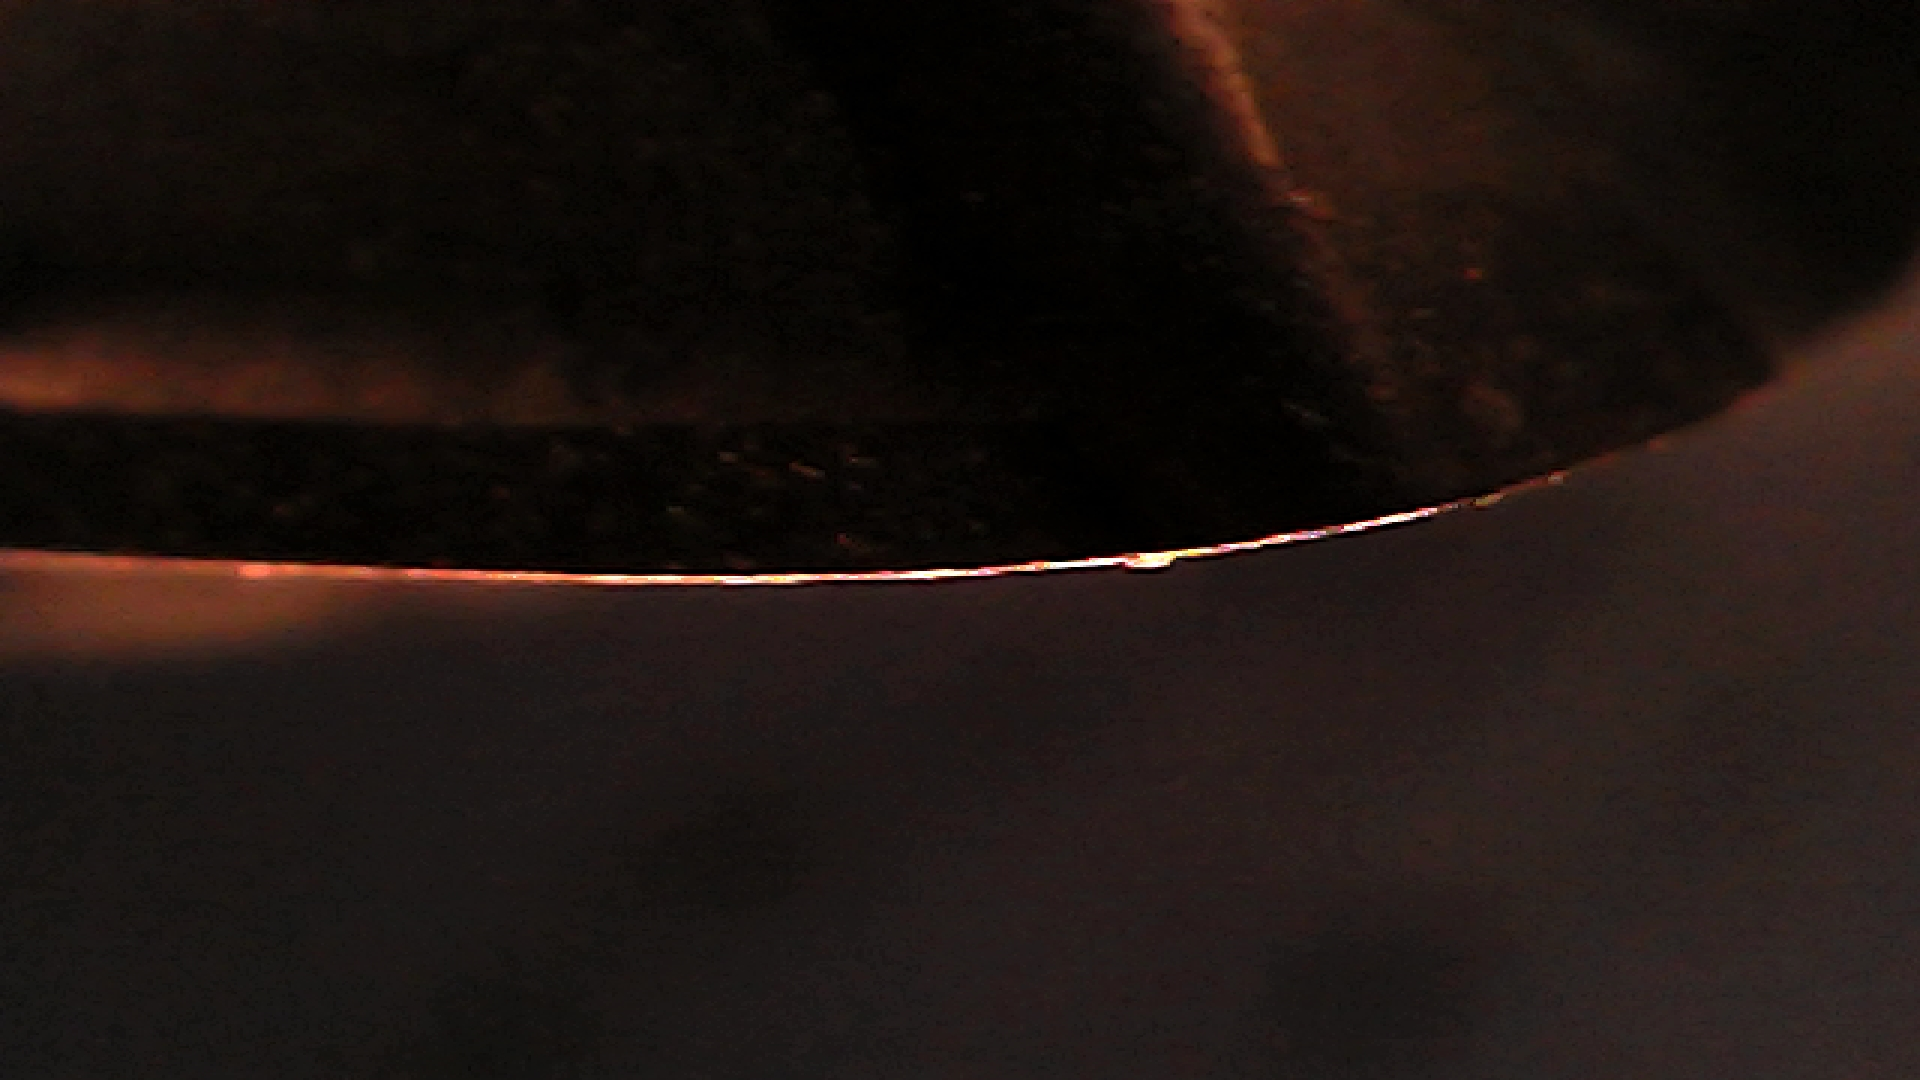
\includegraphics[width=4.166667in, keepaspectratio=true]{./Masterproef_Tool_Wear_Inspection_-_Update_2_DH/eerste-opstelling_donkere_achtergrond3.jpg}





Begin van een setup met een rad waar 20 plaatjes op gemonteerd kunnen worden. Hiervoor heb ik al een 3D model geprint en ben ik gestart aan de aansturing van de motor. Voor de motor heb ik ook berekend dat ik nog een stapreductie zal moeten doen van ongeveer 4:1 gezien een stap van de motor die ik heb (NEMA17) momenteel 1,7mm bedraagt op de rand van het rad. Dit wil ik hiermee terugbrengen tot 0,4mm zodat de plaatjes nauwkeurig voor de camera geplaatst kunnen worden. Ik dacht hiervoor een set van tandwielen zelf te 3D printen. Een foto van de opstelling is te zien in de bijlage.

A close up of a device



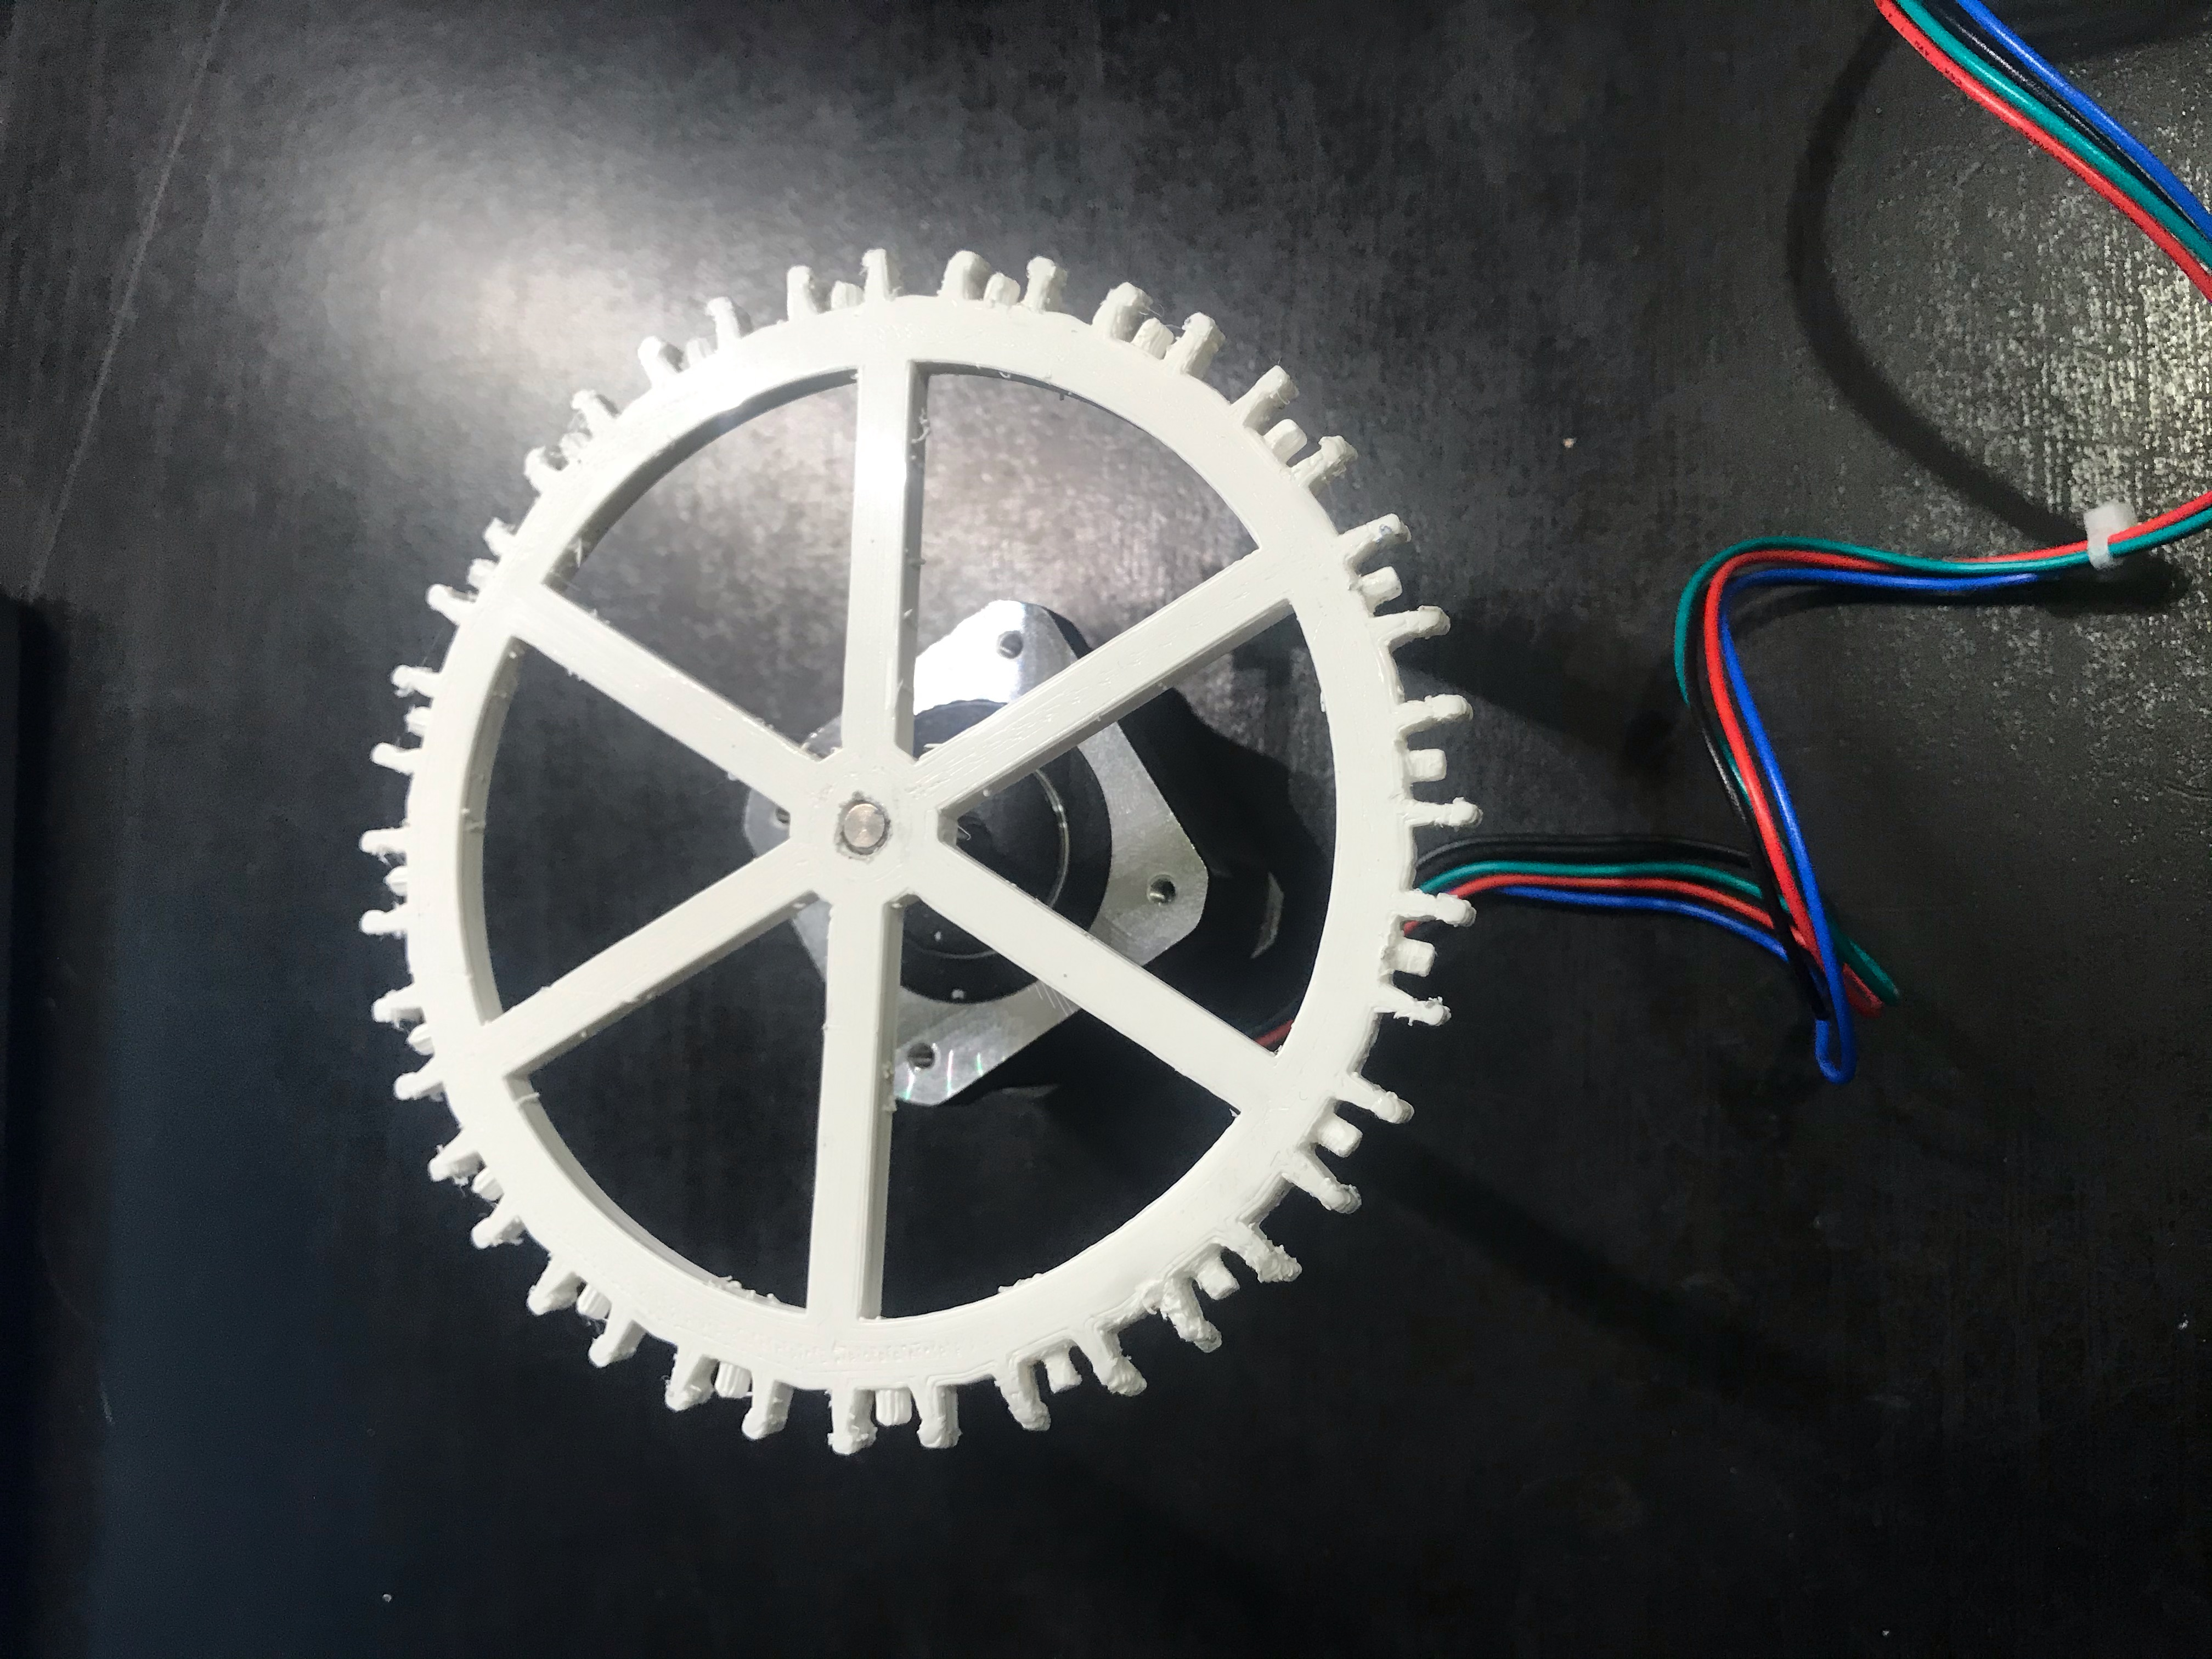
\includegraphics[width=4.166667in, keepaspectratio=true]{./Masterproef_Tool_Wear_Inspection_-_Update_2_DH/radhouder_horizontal.jpeg}

Bekijken welke lichten beschikbaar zijn.

Lange stevige led strips wit licht van ongeveer 30cm. Deze kunnen worden aangestuurd met een relais vanaf de raspberry pi, maar met mijn Solid State relais gaf dit een zeer vreemd gedrag. Bij het uitschakelen bleven de leds gewoon branden en was er een weerstand te meten van enkele mega Ohm. Daarom heb ik geprobeerd met een gewone aanstuurbare relais en dit werkte wel, maar hier heb ik er slechts één van. Ik heb nog een andere opstelling voor deze ledstrips getest door transistoren te gebruiken als switch, maar hier denk ik de foute transistoren gebruikt te hebben. Daar heb ik geen verdere berekeningen rond gedaan gezien dat niet het doel is van het onderzoek. Daarom mijn vraag: zijn er enkele (3) relais beschikbaar op de campus die ik zou kunnen gebruiken of kunnen er eventueel besteld worden? Ik heb er indien nodig zelf 3, maar dan moet ik die uit andere projecten halen.

De adresseerbare led strip heb ik nog niet kunnen testen.

Documenteren van alle afgelopen tests en opstellingen in zim (uitgezonderd software). Dit is allemaal geschreven in het engels om mezelf te verplichten om wat meer na te denken over de woorden en zinnen in het engels om later vlotter te kunnen schrijven aan de thesis tekst.

De Zim bestanden staan publiek op github: \href{https://github.com/dplars/TWI_zim.git}{https://github.com/dplars/TWI\_zim.git}

Is het voor u handig om de zim notebook zelf te openen of stuur ik hier best een samenvatting van?

 

Wat ik komende week zou willen doen:

Langsgaan bij Tom Jacobs voor de extra 300 plaatjes en enkele vragen.

De opstelling met het rad afronden voor de camera en de plaatjes zonder belichting.

De invloed van de lichtkleur op de plaatjes onderzoeken als ik weet uit welke materialen de plaatjes bestaan en of de plaatjes allemaal uit hetzelfde materiaal bestaan.

 

Wat we vorige keer hadden besproken:

Opstelling

3D printen

Verschillende kanten belichten en in channels van de foto zetten

Wanneer de fouten die voorkomen in de plaatjes gekend zijn beoordelen of de resolutie van de camera hoog genoeg is.

Licht

Onderzoeken of er bepaalde reacties zijn van de materialen op golflengtes

Hiervoor en voor de verschillende belichtingshoeken gebruikmaken van adresseerbare led strip

Andere punten

Vooral veel testen en goed documenteren, het echte schrijven komt later pas

Een binair classificatie model gebruiken om de verschillende camera setups snel te kunnen testen.

Eventueel de grootste reflectie blob uitsnijden om de achtergrond weg te kunnen werken.

 

Herhaling van de vragen:

Zijn er 3 relais beschikbaar om de lichten mee te kunnen aansturen?

Zim delen via github of een samenvatting geven?

 

 

Met vriendelijke groeten,

 

Lars De Pauw



\subsection{Reply}

Beste Lars,



Dat ziet er al zeer goed uit! Als we met bepaalde kleuren gaan werken kunnen we de slijtage ook nog beter afzonderen van de rest van de foto.



Als je wil kan ik je relais opsturen maar ik zou eerder opteren om de ledstrips met mosfets te schakelen om dat klikgeluid niet altijd te hebben. Die kan ik ook bij jou laten leveren als je wil? Laat maar weten wat voor jou het beste lijkt.



Het rad ziet er ook zeer goed uit! In fusion360 heb je plugins voor tandwielen te genereren, welk tekenprogramma gebruik je juist?



Ik ben benieuwd als je de plaatjes op het rad zet en ze voorbij de camera laat draaien of de hoek van het licht dan perfect is voor elk plaatje, of dat je onder verschillende hoeken moet belichten. Maar dat kunnen we dan zien als die setup up and running is.



Goed bezig en succes!



\subsection{Mail}

Beste meneer Hulens,

 

Ik heb intussen nog mosfets gevonden thuis en kan de leds hiermee aansturen.

 Fusion 360 is inderdaad gebruikt geweest om de 3D modellen te tekenen. Echter heb ik na het testen gemerkt dat ik de motordriver driver kan instellen om tot 1/16 van een stap te bewegen, waardoor de tandwielen niet meer nodig zijn.

 

De testopstelling is bijna klaar nu, enkel nog de camera monteren en dan kan ik beginnen kijken naar het effect van het licht op de beelden.

 

Woensdag heb ik afgesproken met Tom Jacobs, hij kan nog 90 gelabelde plaatjes (180 snijkanten) voorzien.

 

Met vriendelijke groeten,

 

Lars De Pauw



\end{document}
